
%%%%%%%%%%%%%%%%%%%%%%%%%%%%%%%%%%%%%%%%%%%%
\section{Ultrasound Needle Tracking}


\begin{frame}
  \frametitle{Table of Contents}
  \tableofcontents[currentsection]
\end{frame}



% \subsection{Clinical background}

% %%%%%%%%%%%%%%%%%%%%%%%%%%%%%%%%%%%%%%%%%%%%%%%%%%%%%%%%
% {
% \paper{
% Wright-Gilbertson M. 2014 in PhD thesis; \url{https://en.wikipedia.org/wiki/Gestational_age}; 
% National-Health-Service 2021. Screening for down’s syndrome, edwards’ syndrome and patau’s syndrome. \url{https://www.nhs.uk/pregnancy/your-pregnancy-care} 
% }

% \begin{frame}{Dating US scan (12-week scan)}
%       \begin{figure}
%         \centering
%         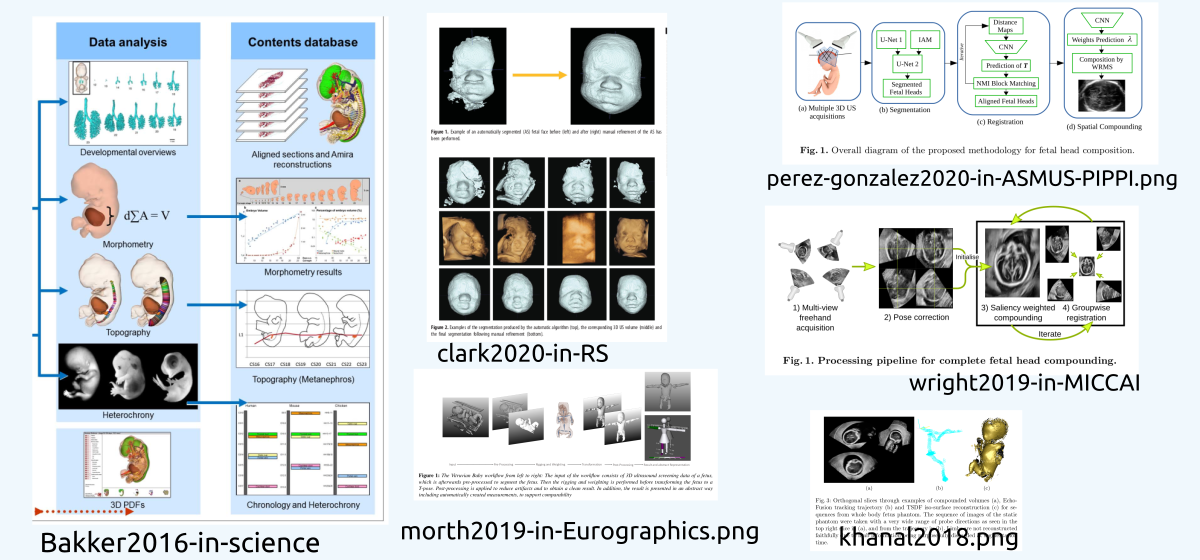
\includegraphics[width=1.0\textwidth]{12-week-scan/versions/drawing-v01}
%         % \caption{The sonographer-probe-patient control system}
%       \end{figure}
% \end{frame}
% }



%%%%%%%%%%%%%%%%%%%%%%%%%%%%%%%%%%%%%%%%%%%%%%%%%%%%%%%%
{
\paper{
  Baker, Christian; Xochicale, Miguel; et al. 
  % Fang-Yu Lin, Sunish Mathews, Francois Joubert, Dzhoshkun I. Shakir, Richard Miles, Charles A. Mosse, Tianrui Zhao, Weidong Liang, Yada Kunpalin, Brian Dromey, Talisa Mistry, Neil J. Sebire, Edward Zhang, Sebastien Ourselin, Paul C. Beard, Anna L. David, Adrien E. Desjardins, Tom Vercauteren, and Wenfeng Xia. 2022.
   "Intraoperative Needle Tip Tracking with an Integrated Fibre-Optic Ultrasound Sensor" Sensors 22, no. 23: 9035. https://doi.org/10.3390/s22239035
}
\begin{frame}{Intraoperative Needle Tip Tracking (2019-2021) @ KCL}
      \begin{figure}
        \centering
        \includegraphics[width=1.0\textwidth]{unt/versions/drawing-v00}
        % \caption{The sonographer-probe-patient control system}
      \end{figure}
\end{frame}
}





%%%%%%%%%%%%%%%%%%%%%%%%%%%%%%%%%%%%%%%%%%%%%%%%%%%%%%%%
{
\paper{
  Xochicale Miguel et al. 
  Finding a fETus with UltraSound (FETUS); \faGithub    https://github.com/xfetus/pe 
}
\begin{frame}{Finding a fETus with UltraSound (FETUS) (2019-2021) @ KCL}
      \begin{figure}
        \centering
        \includegraphics[width=1.0\textwidth]{fetus/versions/drawing-v00}
        % \caption{The sonographer-probe-patient control system}
      \end{figure}
\end{frame}
}






% \subsection{Research aims}


% %%%%%%%%%%%%%%%%%%%%%%%%%%%%%%%%%%%%%%%%%%%%%%%%%%%%%%%%
% {
% %\paper{Wright-Gilbertson M. 2014 in PhD thesis}
% \begin{frame}{Research aims}	
% \begin{itemize}
% \item Investigate and implement deep-learning methods for synthetic fetal ultrasound imaging of normal and abnormal cases;
% \item Propose and apply methods to evaluate quantitative and qualitative images to investigate fetal biomechanics; and 
% \item Design and  test fetal phantoms that mimic various poses, and fetal ages.
% % \item 
% \end{itemize}

% \end{frame}
% }

